\begin{frame}
    \frametitle{Outline} 
    \tableofcontents[currentsection]
\end{frame} 

\begin{frame}
    \frametitle{Main Research Question} 

    \vspace{-0.7cm}
    \begin{center}
        \LARGE{How sensitive are \ce{O3} concentrations to non-chemical variables?}
    \end{center}
\end{frame}

\begin{frame}
    \frametitle{1. Tagging Approach}

    \begin{itemize}
        \item VOC tagging approach implemented in global model by Shuai and Tim.
        \item Allows allocation of \ce{O3} mixing ratios to source rather than comparing \ce{O_x} production.
        \item Tagged MOZART-4 mechanism that was implemented in boxmodel for mechanism comparison study.
        \item Same boxmodel set-up as in mechanism comparison study.
    \end{itemize}
\end{frame}

{
    \usebackgroundtemplate{%
        \vbox to \paperheight{\vfil\hbox to \paperwidth{\hfil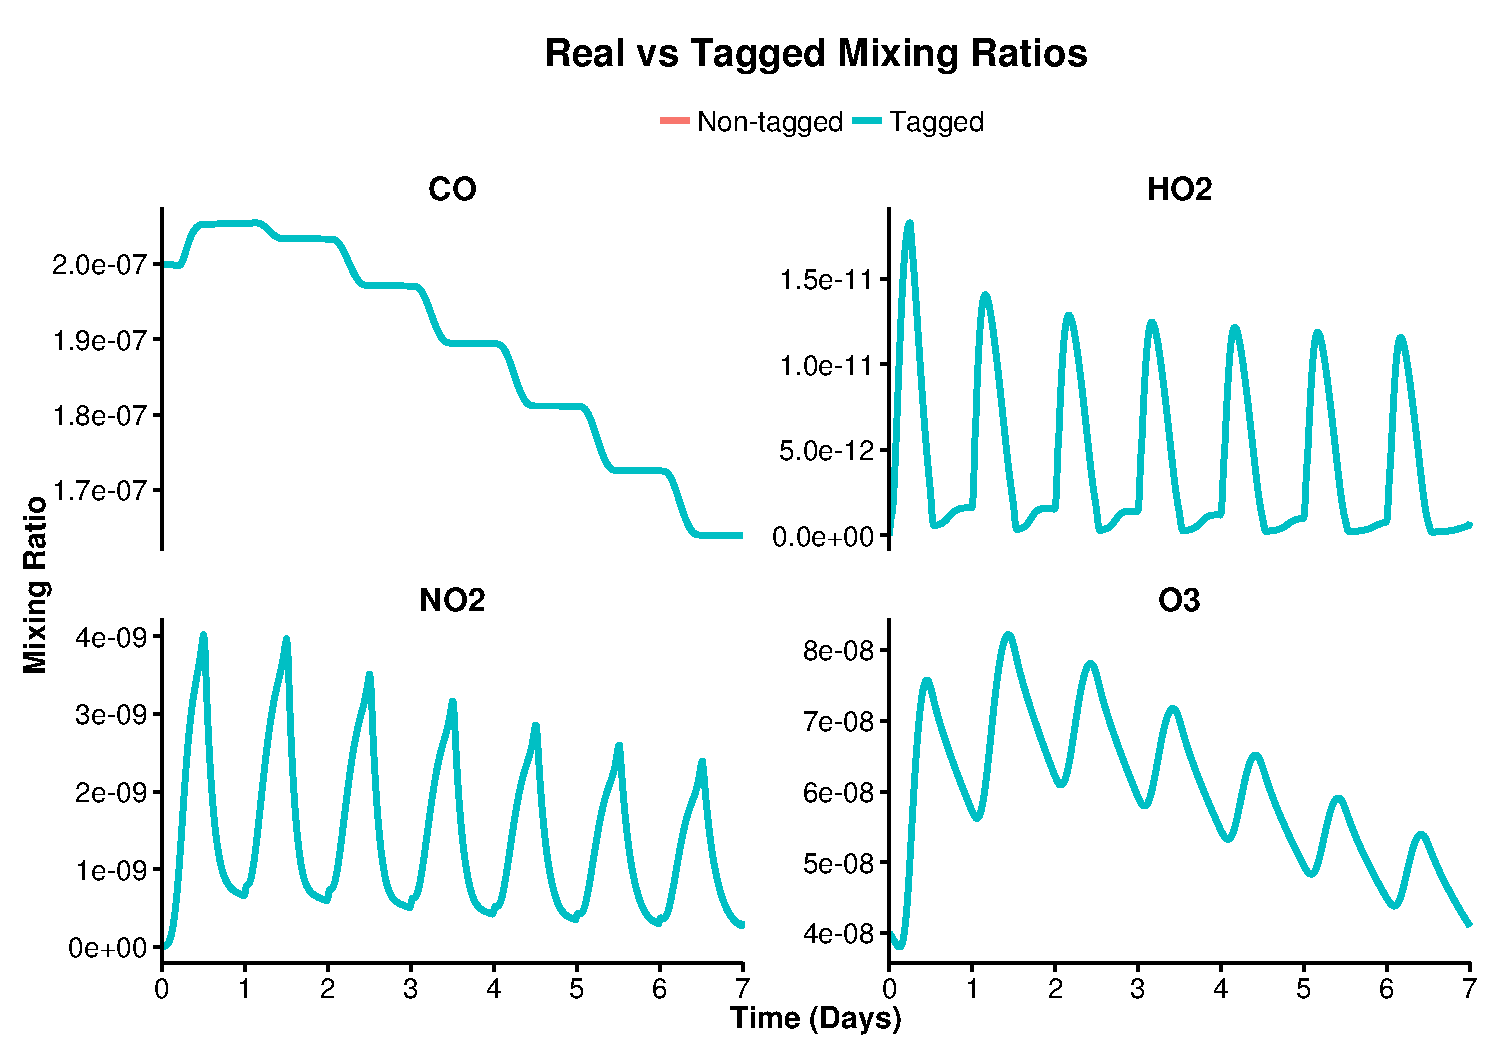
\includegraphics[height=0.90\paperheight, width = 0.98\paperwidth]{../Plotting_scripts/tagged_non-tagged_mixing_ratios}\hfil}\vfil}
    }
    \begin{frame}[plain]
    \end{frame}
}

{
    \usebackgroundtemplate{%
        \vbox to \paperheight{\vfil\hbox to \paperwidth{\hfil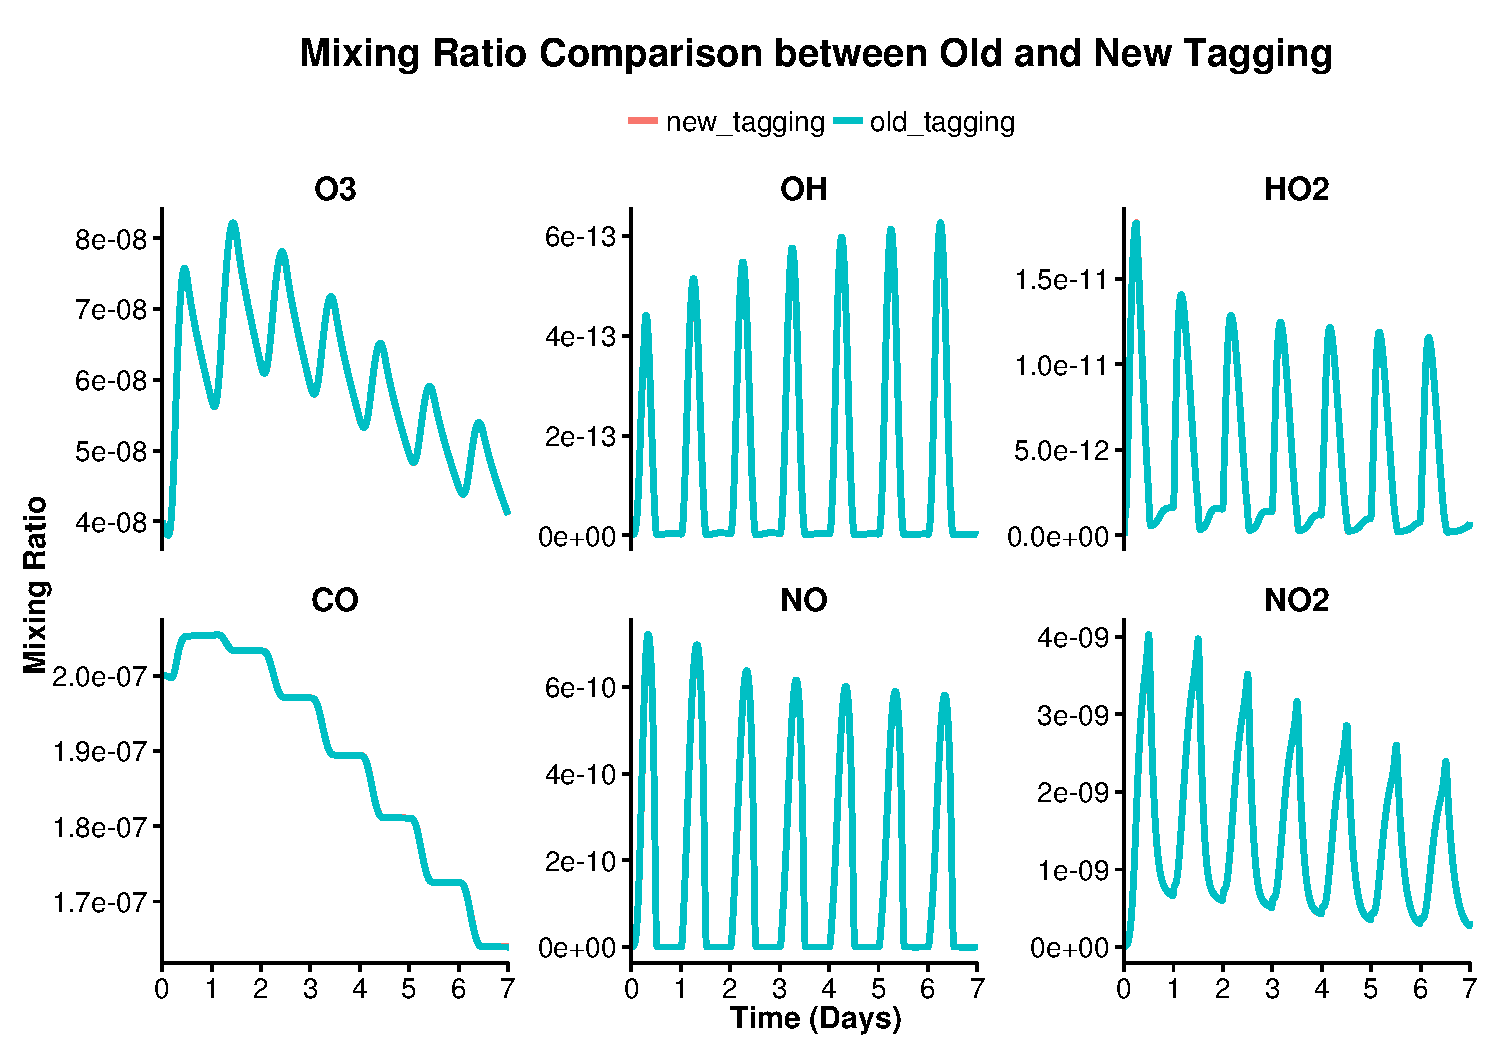
\includegraphics[height=0.90\paperheight, width = 0.98\paperwidth]{../Plotting_scripts/old_vs_new_tagging_mixing_ratios}\hfil}\vfil}
    }
    \begin{frame}[plain]
    \end{frame}
}

{
    \usebackgroundtemplate{%
        \vbox to \paperheight{\vfil\hbox to \paperwidth{\hfil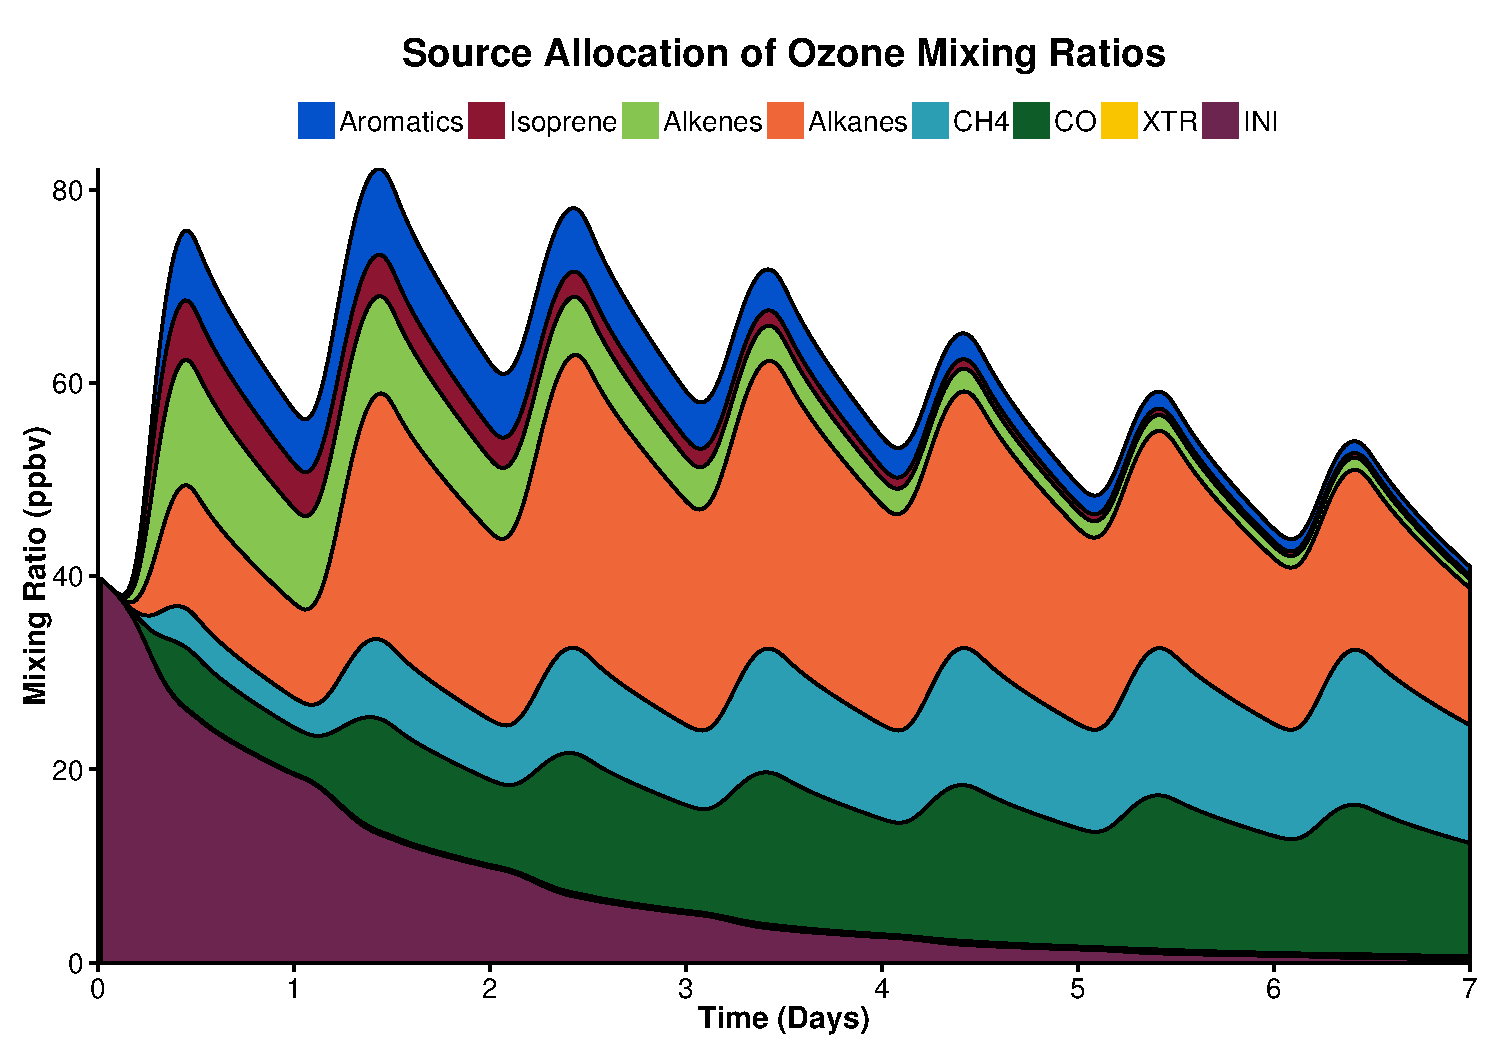
\includegraphics[height=0.90\paperheight, width = 0.98\paperwidth]{../Plotting_scripts/O3_mixing_ratio_components}\hfil}\vfil}
    }
    \begin{frame}[plain]
    \end{frame}
}

\begin{frame}
    \frametitle{2. Low and High \ce{NO_x} Conditions}

    \begin{itemize}
        \item Modelling rural (low) and polluted urban (high) \ce{NO_x} conditions.
        \item MOZART-4 mechanism with VOC tagging approach.
        \item Same VOC emissions and boxmodel set-up as in mechanism comparison study.
        \item NO emissions calculated for maximum \ce{O3} production scaled by
            \begin{itemize}
                \item 0.5 for Low \ce{NO_x}
                \item 1.5 for High \ce{NO_x}
            \end{itemize}
    \end{itemize}
\end{frame}

{
    \usebackgroundtemplate{%
        \vbox to \paperheight{\vfil\hbox to \paperwidth{\hfil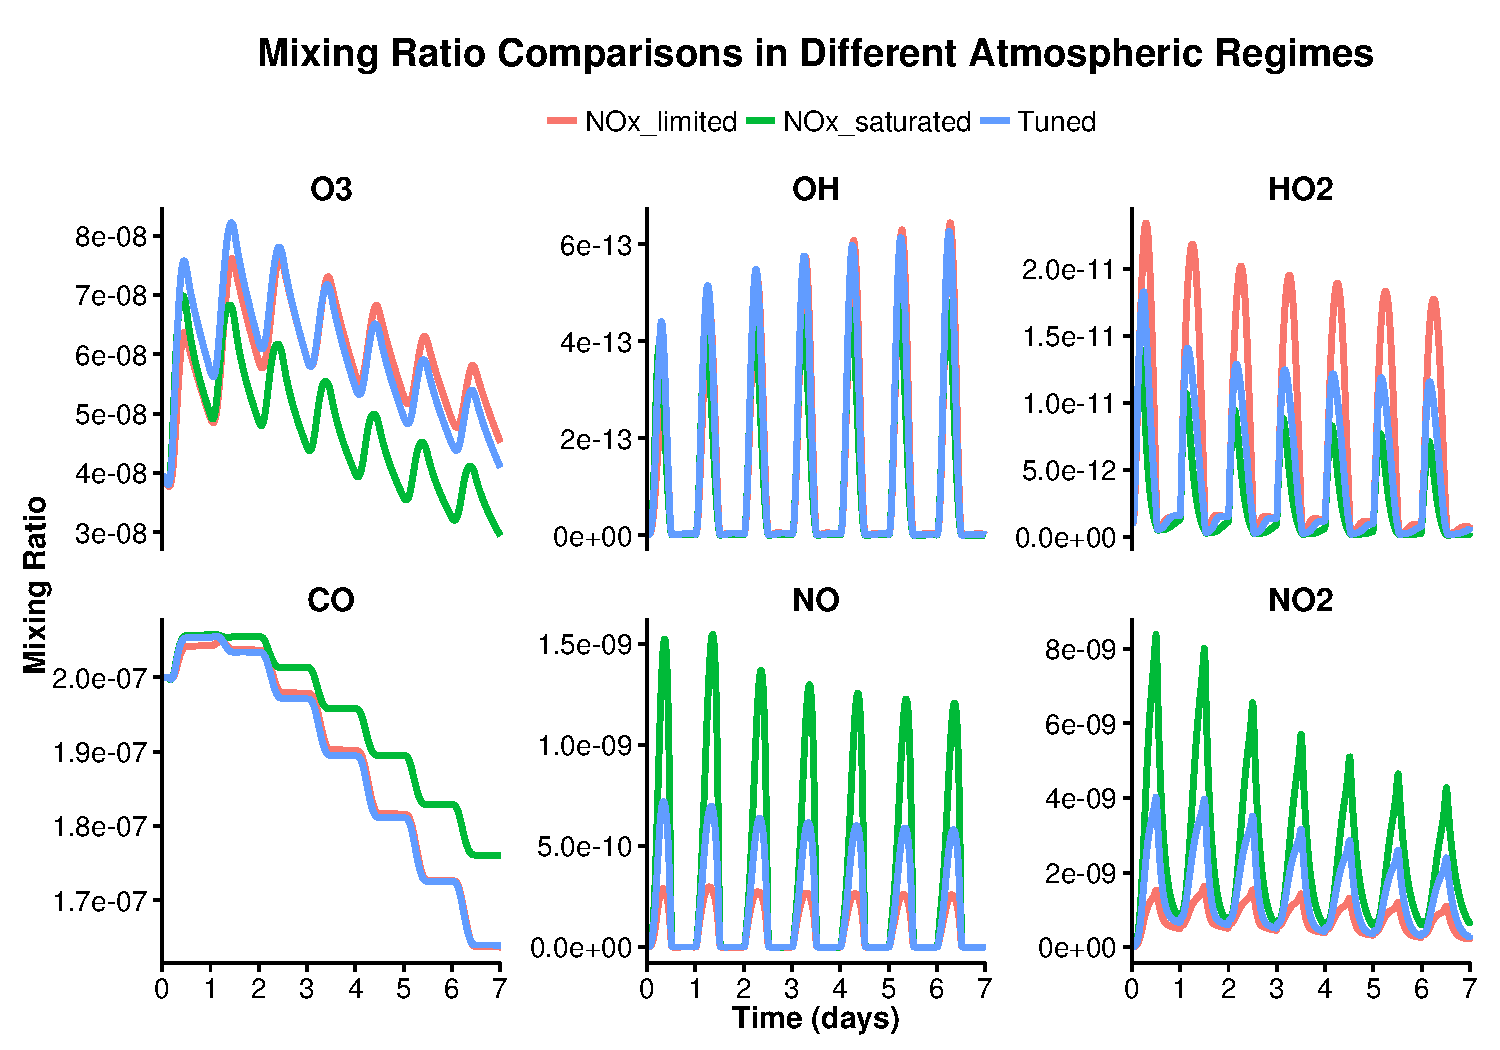
\includegraphics[height=0.90\paperheight, width = 0.98\paperwidth]{../Plotting_scripts/low_high_nox_non-tagged_mixing_ratios_comparison}\hfil}\vfil}
    }
    \begin{frame}[plain]
    \end{frame}
}

{
    \usebackgroundtemplate{%
        \vbox to \paperheight{\vfil\hbox to \paperwidth{\hfil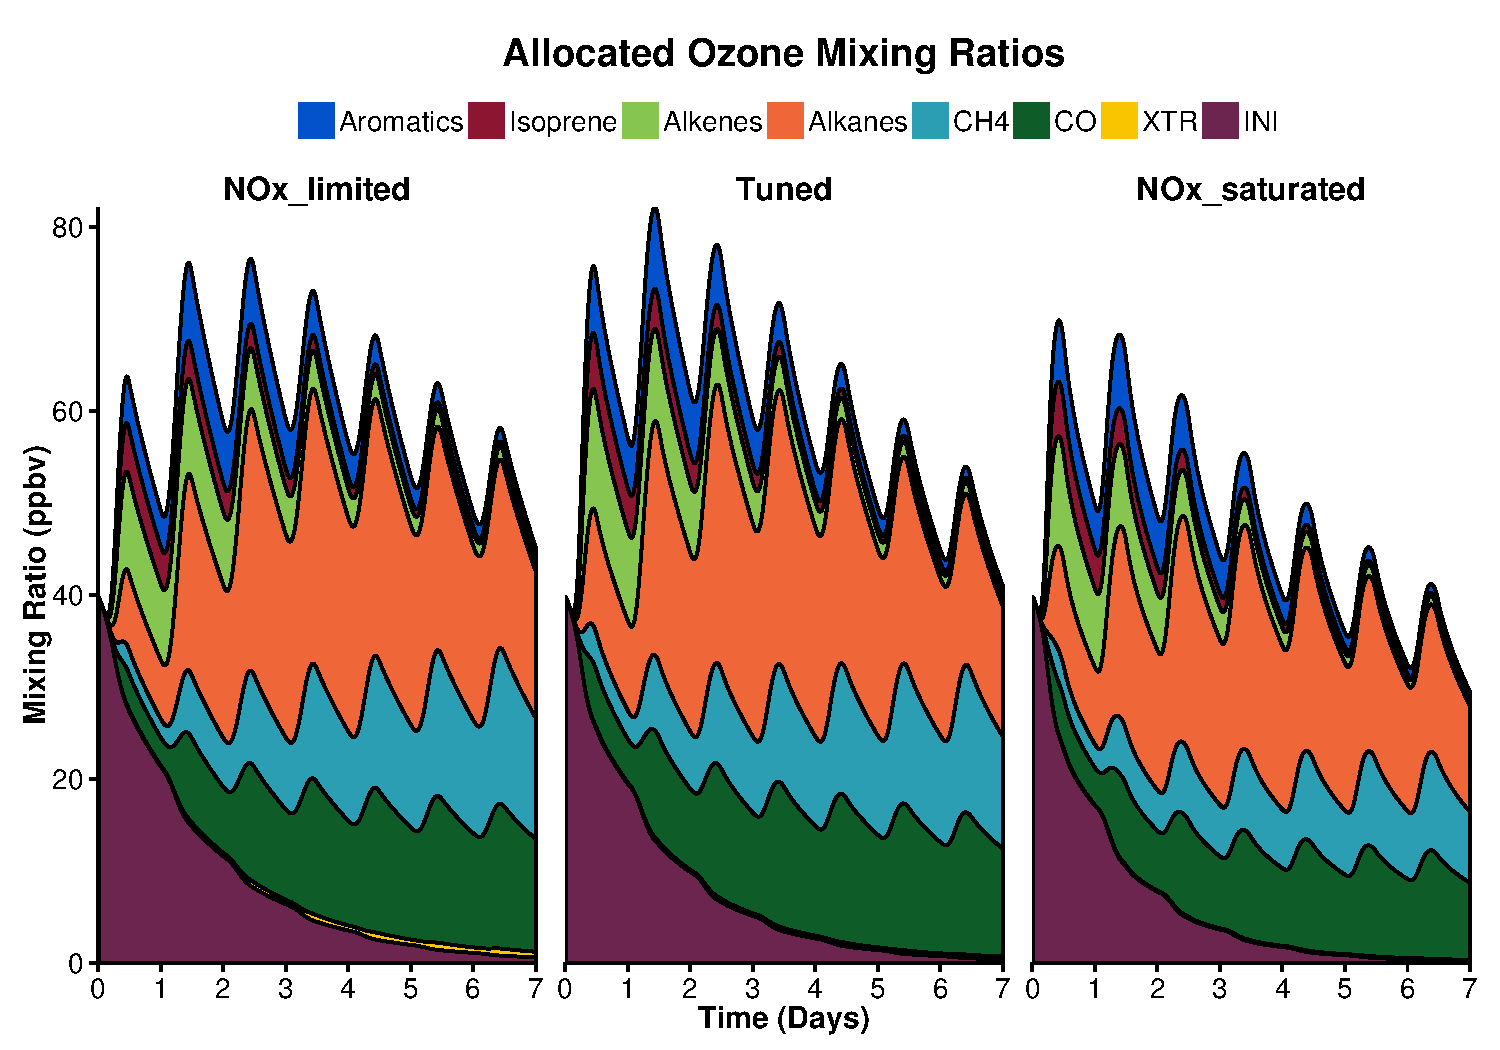
\includegraphics[height=0.90\paperheight, width = 0.98\paperwidth]{../Plotting_scripts/low_high_nox_O3_mixing_ratio_components_facet_run}\hfil}\vfil}
    }
    \begin{frame}[plain]
    \end{frame}
}

\begin{frame}
    \frametitle{3. Vertical Mixing}

    \begin{itemize}
        \item Same boxmodel set-up as VOC tagging approach.
        \item Initial VOC are kept constant till noon of the first day.
        \item Included diurnal cycle for PBL height.
        \item Vertical mixing with free troposphere approach as in Sandra Louren's thesis.
        \item Free troposphere mixing ratios for \ce{O3} and CO from MATCH-MPIC model.
    \end{itemize}
\end{frame}

{
    \usebackgroundtemplate{%
        \vbox to \paperheight{\vfil\hbox to \paperwidth{\hfil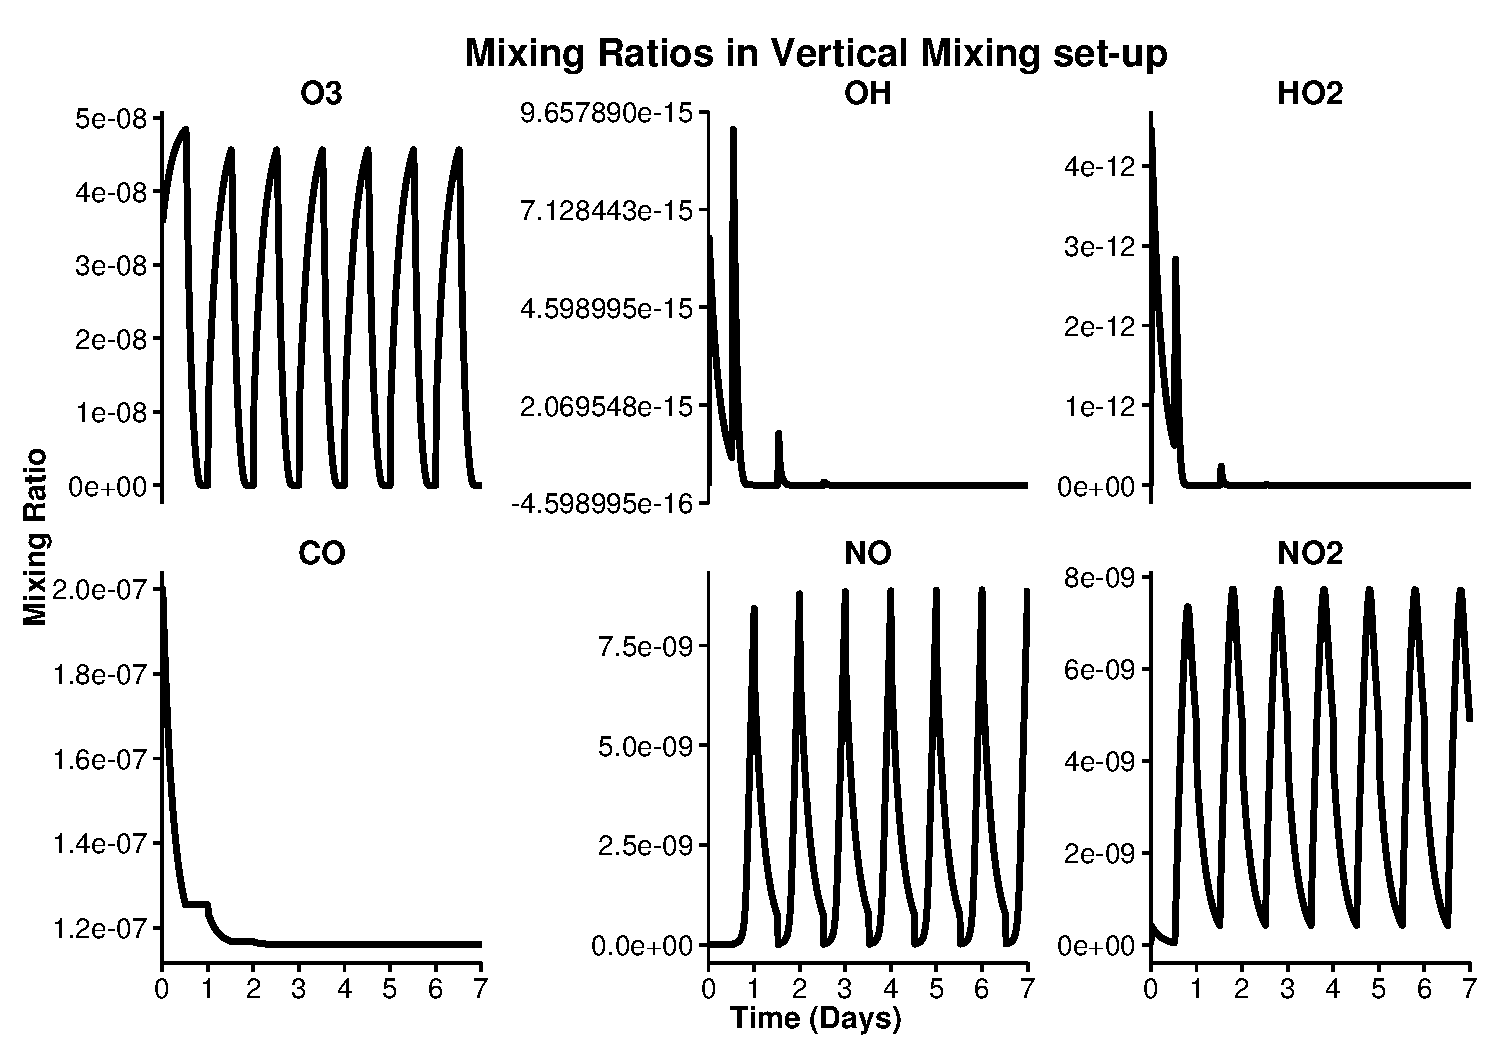
\includegraphics[height=0.90\paperheight, width = 0.98\paperwidth]{../Plotting_scripts/vertical_mixing_mixing_ratios}\hfil}\vfil}
    }
    \begin{frame}[plain]
    \end{frame}
}

\begin{frame}
    \frametitle{4. Horizontal Mixing}

    \begin{itemize}
        \item Same boxmodel set-up as VOC tagging approach.
        \item Implement horizontal mixing approach as in Sandra Louren's thesis.
        \item ??? what is the modelling case?
    \end{itemize}
\end{frame}

\begin{frame}
    \frametitle{5. Temperature}

    \begin{itemize}
        \item Current boxmodel setup uses constant temperature (293 K).
        \item Run boxmodel at 295 K, future scenario of a warmer climate.
        \item Compare \ce{O3} between lower and higher temperatures.
        \item Based on recent review by Pusede et al., temperature impacts \ce{O3} production through chemistry of alkyl nitrates (RONO2) and peroxy nitrates (RO2NO2).
        \item See which chemical mechanisms reflect the temperature dependance of this chemistry and its effect on \ce{O3}.
    \end{itemize}
\end{frame}
